\documentclass[a4paper,12pt]{article}
%%%%%~~~~~~~~~~~~~~~~~~~~~usepackage~~~~~~~~~~~~~~~~~
\usepackage{rotating}
\usepackage[top=0.8in, bottom=0.8in, left=0.8in, right=0.8in]{geometry}
\usepackage{graphicx}
\usepackage[numbers,square,sort&compress]{natbib}
\usepackage{setspace}
\usepackage[cdot,mediumqspace,]{SIunits}
\usepackage{caption}
\usepackage{subcaption}
\usepackage{mathtools}
\usepackage{authblk} % to get affil
\usepackage{float} % to get figures where wanted
\usepackage{indentfirst} % to indent the first para of every chapter use ...\\ \indent
\usepackage{listings} % to add code to the document
\usepackage[toc,page]{appendix} % to add appendix

%####################### new command

\newcommand{\myemail}{ayushi.singh@mail.utoronto.ca}
\newcommand{\anita}{anita.bahmanyar@mail.utoronto.ca}
\newcommand{\carly}{c.berard@mail.utoronot.ca}

%####################### Title and etc

\begin{document}
\onehalfspacing
\title{Astrometry from CCD Images}
\author{Ayushi Singh, Anita Bahmanyar, Morten Nyborg Stostad}
\affil{\small {\myemail}}%, {\anita}, {\carly}}
\affil{\small Astronomy and Physics, University of Toronto, ON}
\date{4 December, 2013}
\maketitle
%\altaffiltext{1}{{\myemail}}
%\altaffilmark{1}
%####################### Abstract #### this is done

\begin{abstract}
\label{abstract}
This experiment examines the five epoch of 30 Urania asteroid to obtain the orbital elements and the model of the orbit. Python programming language and DS9 software was used to inspect, calculate and model the data. The position of asteroid at each epoch, after correcting for plate constants, was obtained in lab 3. However, due to high residuals and high $\chi_{red}^{2}$ for $x$ and $y$, the these position were incorrect. Therefore using positions from JPL Horizons all orbital elements were calculated within small errors. This was used to predict $\alpha$ and $\delta$ at another time: $t = 2455950.68528$, where $\alpha =$ 3:00:18.63, $\Delta\alpha =$ 0:01:18.83 and $\delta =$ +19:23:10.58, $\Delta\delta =$ +0:00:53.11. Similarly, this was done for all five epoch, which showed variation within errors indicating that the result was not very consistent. 

\end{abstract}

%####################### Introduction %%%% this is done
\section{Introduction}
\label{sec:introduction} 
The purpose of this experiment was to find the orbital elements of the 30Urania Asteroid and model the orbit. It was done using the data collected from Dunlap Institute Telescope on five different days and the position of the 30Urania Asteroid in equatorial coordiantes calculated in lab3 \cite{lab3}. The orbit of an object around sun is the path it takes over the course of its period. This object will have six orbital elements that will determine the shape and orientation of the orbit and the period of the object. These elements are: semi-major axis, eccentricity, inclination, longitude of ascending node, epoch of perihelion, and argument of perihelion. These six elements are constants and therefore, can be used to calculate the position of this object at any given time (Julian Day), by calculating true anomaly, mean anomaly and eccentric anomaly. In this lab, all six orbital elements of 30Urania Asteroid are calculated.\\
\indent The report explains the step by step process used to obtain the final result with errors. After observed position of the Asteroid was corrected using plate constants for each epoch, it was converted from equatorial coordiantes into ecliptic coordiantes. Using these position and the distance of Earth from sun from JPL \cite{jpl}, all the six orbital elements were calculated and the orbit of asteroid was modelled.   

%####################### Equipment %%%% this is done
\section{Equipment}
\label{sec:equipment} 
The data was collected using Dunlap Institute Telescope (DIT) that was located at New Mexico Skies on Mt. Joy site near Mayhill, NM. It was a 50-cm robotic telescope dedicated to the search for optical counterparts of gamma-ray bursts. The telescope had 4096 $\times$ 4096 pixel CCD array, with the view of 36 $\times$ 36 arc minutes. The focal length being 3454 mm and with F/ratio = F/6.8 \cite{instructions}. Also, an online catalog was used for the obtaining the position of Earth from Sun at each epoch. This catalog is called JPL's Horizons web-interface \cite{jpl}. It was also used to check the accuracy of our results. For the data reduction, calculations and modelling, DS9 software and Python Programming Language was used. DS9 provided the visual representation of the data set, including all the statistic about the data in the header. And Python allowed to perform calculations and modelling of the data. 

%####################### Data %%%% this is done
\section{Data Summary}
\label{sec:data}

The data was already collected before hand and the link to the data was provided to us at the start of this experiment on the course website \cite{instructions}. 


\begin{table}[H]
\centering % used for centering table
\caption{Summary of all the data collected for this experiment}
\tabcolsep 2.pt %\small
\footnotesize

\begin{tabular}{ccccccc}% centred columns (8 columns)
\hline
\hline
Data \# & Name & Date & Time & Julian Date &Comments \\
& &  DD/MM/YYYY&[UTC time]&&\\
\hline
\hline
1   &   30 Urania    & 20/01/2012   &04:28:30&2455946.68646& Asteroid\\
2   &   30 Urania     &  21/01/2012   &04:40:27&2455947.69476&Asteroid \\
3   &    30 Urania   &23/01/2012    &05:43:40 &2455949.73866&Asteroid \\
4   &   30 Urania    & 24/01/2012    &04:26:48&2455950.68528& Asteroid\\
5   &  30 Urania  &  29/01/2012   &01:27:18 &2455955.56062&Asteroid \\
\hline
\hline

\end{tabular}
\label{table:dataset} % is used to refer this table in the text
\end{table}

Each dataset has 3 files provided in them. This includes, raw data, dark counts due to CCD and flat-field taken at either dawn or twilight. The flat-field has already been corrected. 
%####################### Data Reduction and Method %%%%%% edit this 
\section{Data Reduction and Method}
\label{sec:reduction}

%\subsection{Correction for Dark and Flat-field}
%\label{sec:dark}
%The raw data for 30 Urania, from Table \ref{table:dataset},is given as a fits files. Using python module pyfits, the data from the files was extracted. It is in the form of 2-D image with 2048 $\times$ 2048 pixels. Initially, the data is flipped %in a way, that North is pointing down and East is pointing left. This is due the telescope, which records the inverted image. Therefore, the first step was to correct the image so that North is pointing up and East is pointing right. Then, to correct the data following equation was used:

%\begin{equation}
%\label{eq:flat}
%\begin{array}{rcl}
%    I_i &= \frac{R_i - D_i}{F_i} 
%\end{array}
%\end{equation}
%Where $I_i$ is the corrected intensity value for the the pixel number $i$, which is calculated using the raw data ($R_i$), the dark counts ($D_i$) and the flats ($F_i$). However, Equation \ref{eq:flat} is not sufficient for the flat is not correct. The median of flat is $\sim$0.8, which should be 1. Therefore, the whole flat data set is divided by the median of the flat data set. This then gives us the corrected $F_i$.   

\subsection{Positions of the Asteroids}
\label{sec:position}
The first was to extract the position of the asteroid at each epoch, Table \ref{table:dataset}, from the data file using the software DS9. It was done by comparing the patten between each dataset and finding one object that seem to move with respect to the background pattern. Then using python centroids were found for each epoch and was compares with USNO catalog. Using the method described in detail in AST356 Lab 3 \cite{lab3}, plate constants were derived for each file. These constants were derived again because in the lab 3, it was wrongly assumed that one plate constants can be used for all five epoch. Therefore, in this lab, each one were calculated separately and used to get the correct position of the 30 Urania at each day. 
%~~~~~~~~~~~~~~~~~~~~~~~~~~~~~~~~~~~~~~~~~~~~
\begin{table}[H]
\centering % used for centering table
\caption{Comparing Right Ascension and Declination of Urania over 5 epochs.}
\tabcolsep 2.pt %\small
\footnotesize
\begin{tabular}{ccccccc}% centred columns (8 columns)
\hline
\hline
Date  & $\alpha$ & $\delta$ & $\alpha$ (JPL) & $\delta$(JPL) & $\Delta \alpha$ & $\Delta \delta$ \\
& [hms J2000]&[dms J2000] &[hms J2000]&[dms J2000]&[s]&[s]\\
\hline
\hline
20 & 2:57:49.32& +19:14:30.75 &2:57:49.20& +19:14:30.6&0.12&0.69\\
21 & 2:58:44.60& +19:16:27.53 &2:58:44.52& +19:16:46.1&0.08&18.57\\
23 & 3:00:42.06& +19:21:40.13 &3:00:41.30& +19:21:39.6&0.76&0.53\\
24 & 3:01:37.54& +19:23:44.52 &3:01:37.46& +19:23:03.7&0.08&40.82\\
29 & 3:07:02.81& +19:38:13.85 &3:07:01.64& +19:38:19.4&1.17&5.55\\


\hline
\hline
\end{tabular}
\label{table:position} % is used to refer this table in the text
\end{table}
%~~~~~~~~~~~~~~~~~~~~~~~~~~~~~~~~~~~~~~~~~~~~
Table \ref{table:position}, has results from estimated position with corrected plate constants. There are compared with the position from JPL. For $\Delta \alpha$, the values are very small that most are less than a second. However, for $\Delta \delta$, the values are as high as 40.8 s. This is probably the result of the high residuals while calculating plate constants. The $\chi_{red}^2$ value was quite big. For example, for data number 3 from Table \ref{table:dataset}, $\chi_{red}^2$ values are for $\delta$ = 63.30 and $\alpha$ = 0.52, which are quite large. But, it can't be reduced any further.

\subsection{Converting coordiantes}
\label{sec:coordinates}
The position obtained are in equatorial coordinates. First, using the following calculations, $\alpha$ and $\delta$ were converted in cartesian coordinate. 
%~~~~~~~~~~~~~~~~~~~~~~~~~~~~~~~~~~~~~~~~~~~~
\begin{equation}
\label{eq:xyz}
\begin{array}{lll}

x_{eq} = \cos \alpha \cos \delta \\
y_{eq} = \sin \alpha \cos \delta \\
z_{eq} = \sin \delta 

\end{array}
\end{equation}
%~~~~~~~~~~~~~~~~~~~~~~~~~~~~~~~~~~~~~~~~~~~~
Then, they are transformed into ecliptic cartesian coordiantes for further calculation using the following transformation.
%~~~~~~~~~~~~~~~~~~~~~~~~~~~~~~~~~~~~~~~~~~~~
\begin{equation}
\label{eq:conversion}
\begin{array}{rcl}
    \begin{pmatrix}
        x\\ 
        y\\ 
        z
    \end{pmatrix}
=   \begin{pmatrix}
       1 & 0 & 0\\ 
        0& \cos\ \epsilon & \sin\ \epsilon \\ 
        0 & -\sin\ \epsilon & \cos\ \epsilon 
    \end{pmatrix}
=   \begin{pmatrix}
        x_{eq}\\ 
        y_{eq}\\ 
        z_{eq}
    \end{pmatrix}
\end{array}
\end{equation}
%~~~~~~~~~~~~~~~~~~~~~~~~~~~~~~~~~~~~~~~~~~~~
where $\epsilon$ is $23.4392911^{\circ}$. This then forms a unit vector $\bf{s}$ = $[x,y,z]$, representing the distance between asteroid and the Earth.


\subsection{Finding $r$ and $\rho$}
\label{sec:r_rho}
Using $\bf{s}$ for first 3 epoch and following equations $\dot{\bf{s}}$ and $\ddot{\bf{s}}$ for second epoch was calculated. 
%~~~~~~~~~~~~~~~~~~~~~~~~~~~~~~~~~~~~~~~~~~~~
\begin{equation}
\label{eq:sdsdd}
\begin{array}{rl}
\vspace{0.3cm}
\dot{\bf{s}}_2 =& \frac{\tau_3(\bf{s}_2-\bf{s}_1)}{\tau_1(\tau_1+\tau_3)} +\frac{\tau_1(\bf{s}_3-\bf{s}_2)}{\tau_3(\tau_1+\tau_3)} \\
\ddot{\bf{s}}_2 =& \frac{2(\bf{s}_3-\bf{s}_2)}{\tau_1(\tau_1+\tau_3)} -\frac{2(\bf{s}_2-\bf{s}_1)}{\tau_3(\tau_1+\tau_3)} 
\end{array}
\end{equation}
%~~~~~~~~~~~~~~~~~~~~~~~~~~~~~~~~~~~~~~~~~~~~
where $\tau_1 = t_2-t_1$ and $\tau_3 = t_3-t_2$, and these $t$ values were used from table \ref{table:dataset}. This method was derived from taylor expansion. Then distance of Earth from Sun on the second epoch was recored to be $\bf{R}$ $ = [-5.005639235484095e-01,  8.476786115155864e-01, -2.723171022212407e-05]$ from JPL Horizons \cite{jpl}.

%~~~~~~~~~~~~~~~~~~~~~~~~~~~~~~~~~~~~~~~~~~~~
\begin{equation}
\label{eq:rrho}
\begin{array}{rl}
    \vspace{0.3cm}
    \rho =& k^2\left ( \frac{1}{R^3} -\frac{1}{r^3}\right )\frac{\dot{\bf{s}} \cdot \left 
        ( \bf{R} \times \bf{s} \right )}{\dot{ \bf{s}}\cdot \left ( \ddot{\bf{s}} \times \bf{s} \right )}\\
    r^2 =& \rho^2 + R^2 +2\rho \bf{R \cdot s}
\end{array}
\end{equation}
%~~~~~~~~~~~~~~~~~~~~~~~~~~~~~~~~~~~~~~~~~~~~
In both of these equation there is $r$ and $\rho$. Therefore, to calculate $r$ and $\rho$ a loop in python was created and iterated over 100 increments, see appendix A for the code. And the result was the following:


%~~~~~~~~~~~~~~~~~~~~~~~~~~~~~~~~~~~~~~~~~~~~
\label{sec:orbit}
\begin{figure}[H]
\centering
	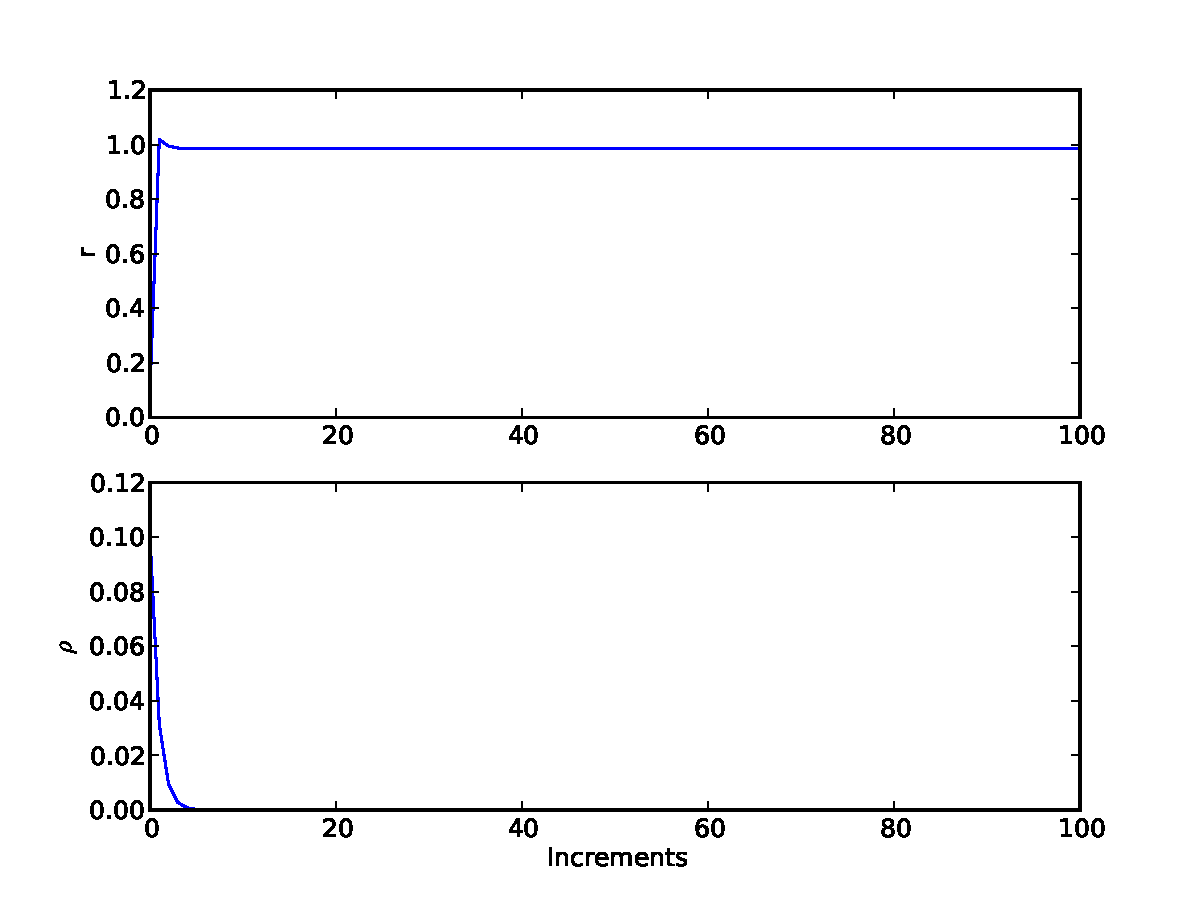
\includegraphics [angle=0,height=7cm,width=9cm]{pic/wrong_rho.pdf} 
\caption{$r$ and $\rho$ value derived using estimated position of Urania.}
\label{fig:wrong}
\end{figure}
%~~~~~~~~~~~~~~~~~~~~~~~~~~~~~~~~~~~~~~~~~~~~
Figure \ref{fig:wrong}, $r$ and $\rho$ converge to 1 and 0, respectively. However, this is not correct for rho being 0 implies that distance better asteroid and Earth is zero. This is because the distance between two is given by $\rho \bf{s}$. Even after many trials, the errors were consistent. They possible reason is discussed in the Section 6.1. So, to continue with the lab and calculate orbital elements, JPL positions were considered, which gave the following result. 

%~~~~~~~~~~~~~~~~~~~~~~~~~~~~~~~~~~~~~~~~~~~~
\label{sec:orbit}
\begin{figure}[H]
\centering
	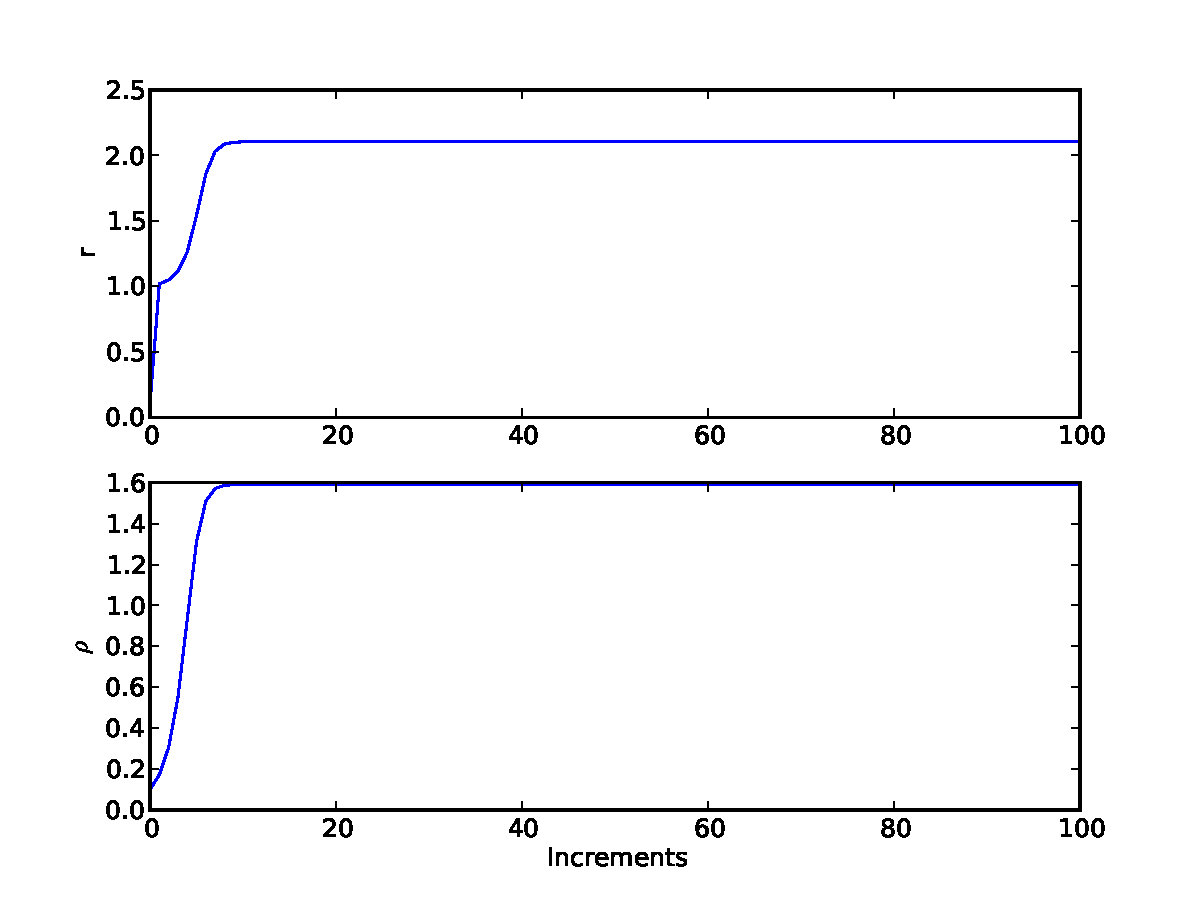
\includegraphics [angle=0,height=7cm,width=9cm]{pic/urania_rho.pdf} 
\caption{$r$ and $\rho$ value derived using JPL position of Urania.}
\label{fig:rho}
\end{figure}
%~~~~~~~~~~~~~~~~~~~~~~~~~~~~~~~~~~~~~~~~~~~~
Figure \ref{fig:rho}, clearly give us a convergence of $r$ to 2.105 and $\rho$ to 1.591. The true value for $r$ and $\rho$ are 2.119 and 1.605, respectively. And the estimated results are within 1\% error. 

%####################### Calculation and Modeling
\section{Calculation and Modelling}
\label{sec:calc}

\subsection{Calculating orbital elements for Urania}
\label{sec:elements}

From $\bf{s}, \bf{R}$ and $\rho$, the following can be calculated
%~~~~~~~~~~~~~~~~~~~~~~~~~~~~~~~~~~~~~~~~~~~~
\begin{equation}
\label{eq:orbital0}
\begin{array}{rl}
\bf{r} =& \bf{R}+ \rho \bf{s}\\
\bf{\ddot{r}} =& \bf{\ddot{R}+\rho \bf{\dot{s}}+\dot{\rho}\bf{s}}\\
\bf{h} =& \bf{r \times \dot{r}} \\

\end{array}
\end{equation}
%~~~~~~~~~~~~~~~~~~~~~~~~~~~~~~~~~~~~~~~~~~~~
Here, $\bf{r}$ is the vector distance between Sun and the asteroid and $\bf{\ddot{r}}$ is the velocity. $\bf{h}$ represents the vector perpendicular to the orbital plane of the asteroid. Now, there are few equations that uses variables from equation \ref{eq:orbital0} to calculate the orbital elements.
%~~~~~~~~~~~~~~~~~~~~~~~~~~~~~~~~~~~~~~~~~~~~
\begin{equation}
\label{eq:orbital1}
\begin{array}{rl}
a =& (k^2r)/(2k^2-rV^2) , V = |\bf{\dot{r}}|^2\\
e =& \sqrt{1-(h^2/ak^2)}\\
\cos i =& h_z/h \\
\tan \Omega =& -h_x/h_y
\end{array}
\end{equation}
%~~~~~~~~~~~~~~~~~~~~~~~~~~~~~~~~~~~~~~~~~~~~
where $a$ is semi-major axis, $e$ is eccentricity, $i$ is inclination, $Omega$ is longitude of ascending node. These gives four of the six elements. Furthermore, using $a$ period of the asteroid can be calculated by $p = 2\pi /n$. Where, $n^2 a^3 = k^2$ and $k = \sqrt{GM_{\odot}}  = 0.017 202 098 950$ AU$^{3/2}$ d$^{-1}$. For Urania, 1263.45 days is the estimated period. Using same method, true period comes to be 1328.44 days. Therefore, there is a error of 64.70 days between true and estimated values.
%~~~~~~~~~~~~~~~~~~~~~~~~~~~~~~~~~~~~~~~~~~~~
\begin{equation}
\label{eq:orbital2}
\begin{array}{rl}
cos E =& a-r/ae\\
M =& E - e sin E \\
\tau =& t - (M/n) \\
\nu =& 2\arctan \left [ \sqrt{\frac{1+e}{1-e}} \tan E/2  \right ]\\
\cos(\nu - \omega) =& (x \cos \Omega + y \sin \Omega)/r
\end{array}
\end{equation}
%~~~~~~~~~~~~~~~~~~~~~~~~~~~~~~~~~~~~~~~~~~~~
here, the last two orbital elements are calculated, $\tau$ is epoch of perihelion and $\omega$ is argument of perihelion. Furthermore, three more equations are also defined in equation \ref{eq:orbital2}. E is eccentric anomaly, M is mean anomaly and $\nu$ is true anomaly. The sign on E is important and need to be placed separately. If the object is going from perihelion to aphelion then E > 0. However, if object is going from aphelion to perihelion then E < 0. In this case, the value of E is kept positive because using the $\bf{\dot{r}}$, it is deduced that asteroid is going from from perihelion to aphelion.


%~~~~~~~~~~~~~~~~~~~~~~~~~~~~~~~~~~~~~~~~~~~~
\begin{table}[H]
\centering % used for centering table
\caption{Comapring true and estimated orbital elements for Urania.}
\tabcolsep 2.pt %\small
\footnotesize
\begin{tabular}{ccccccc}% centred columns (8 columns)
\hline
\hline
  & a & $\Omega$ & i & e & $\omega$ & $\tau$ \\
& [AU]&[deg] &[deg]&&[deg]&[Julian Day]\\
\hline
\hline
True    & 2.365& 307.93 &2.098& 0.127&86.27&2455845.40\\
Estimate& 2.287& 308.26 &2.084& 0.116&74.24&2455802.67\\
Error   & 0.022& -0.33  &0.014& 0.011&12.03&42.73\\
%2455845.40
\hline
\hline
\end{tabular}
\label{table:elements} % is used to refer this table in the text
\end{table}
%~~~~~~~~~~~~~~~~~~~~~~~~~~~~~~~~~~~~~~~~~~~~
This table describes the data estimated and compare it with the true values obtained from JPL. 

\subsection{Modelling the orbit of Urania}

Using the orbital elements and python coding, a model of the asteroid's orbit was created. The time elapse was from $\tau$ to ($\tau$ + period of the orbit + 500 days). 

\label{sec:orbit}
%~~~~~~~~~~~~~~~~~~~~~~~~~~~~~~~~~~~~~~~~~~~~
\begin{figure}[H]
\centering
	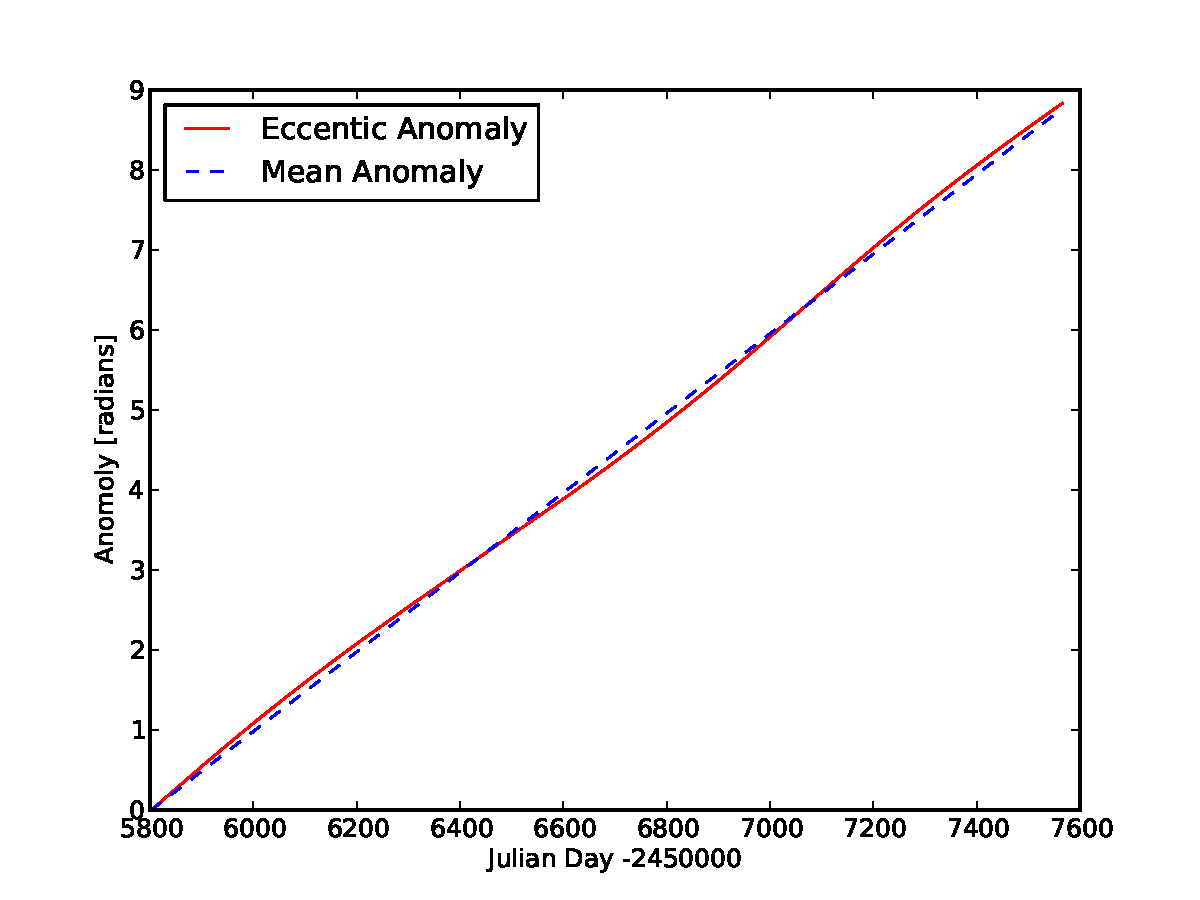
\includegraphics [angle=0,height=5cm,width=7cm]{pic/urania_EM.pdf} 
\caption{Mean anomaly and eccentric anomaly vs. time}
\label{fig:EM}
\end{figure}
%~~~~~~~~~~~~~~~~~~~~~~~~~~~~~~~~~~~~~~~~~~~~
Figure \ref{fig:EM} shows the procession of mean anomaly and eccentric anomaly over time for Urania.
%~~~~~~~~~~~~~~~~~~~~~~~~~~~~~~~~~~~~~~~~~~~~

\begin{figure}[H]
\centering
	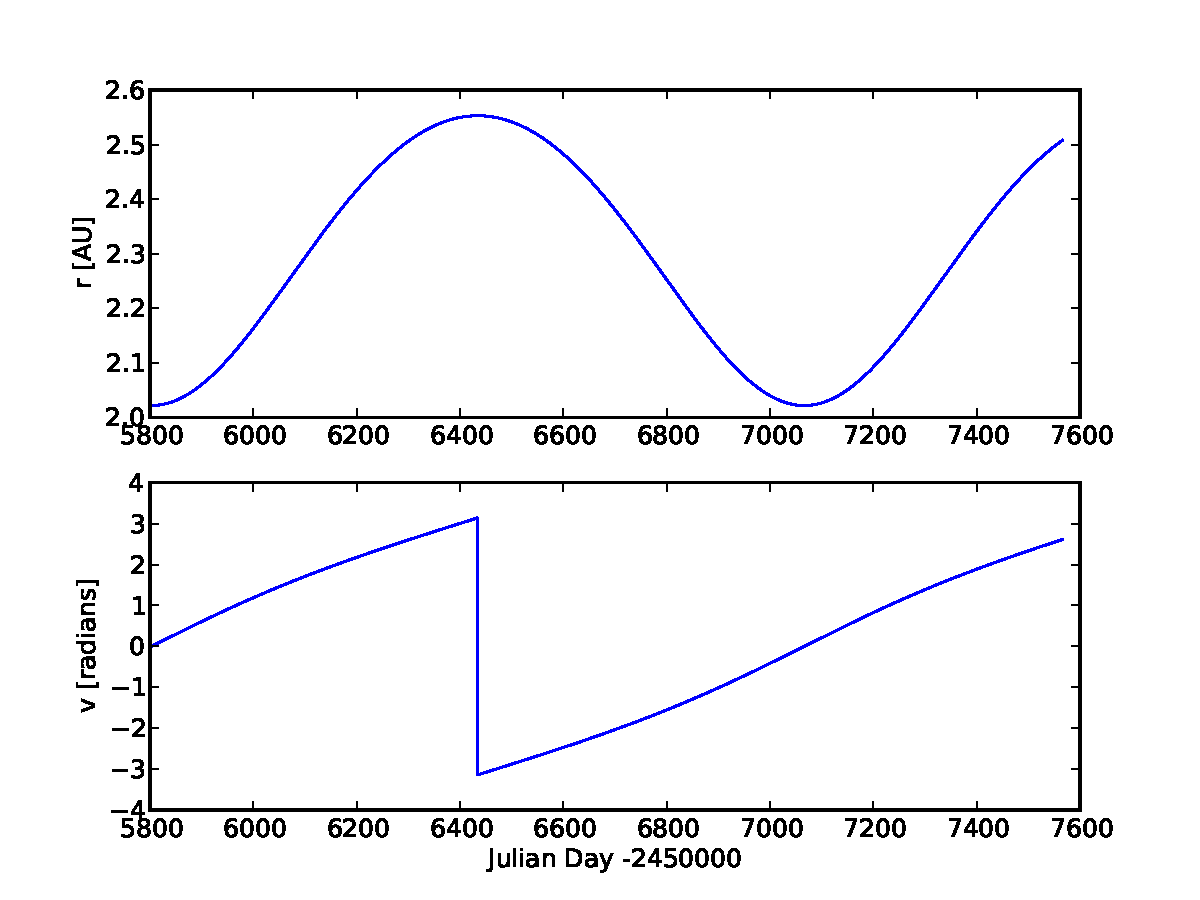
\includegraphics [angle=0,height=6cm,width=9cm]{pic/urania_rv.pdf} 
\caption{Radial sepration and true anomaly}
\label{fig:rv}
\end{figure}
%~~~~~~~~~~~~~~~~~~~~~~~~~~~~~~~~~~~~~~~~~~~~
Figure \ref{fig:rv} shows the radial separation from Sun and the true anomaly, which is the angular distance from $\omega$ as the asteroid moves in it's orbit.

%~~~~~~~~~~~~~~~~~~~~~~~~~~~~~~~~~~~~~~~~~~~~
\begin{figure}[H]
\centering
	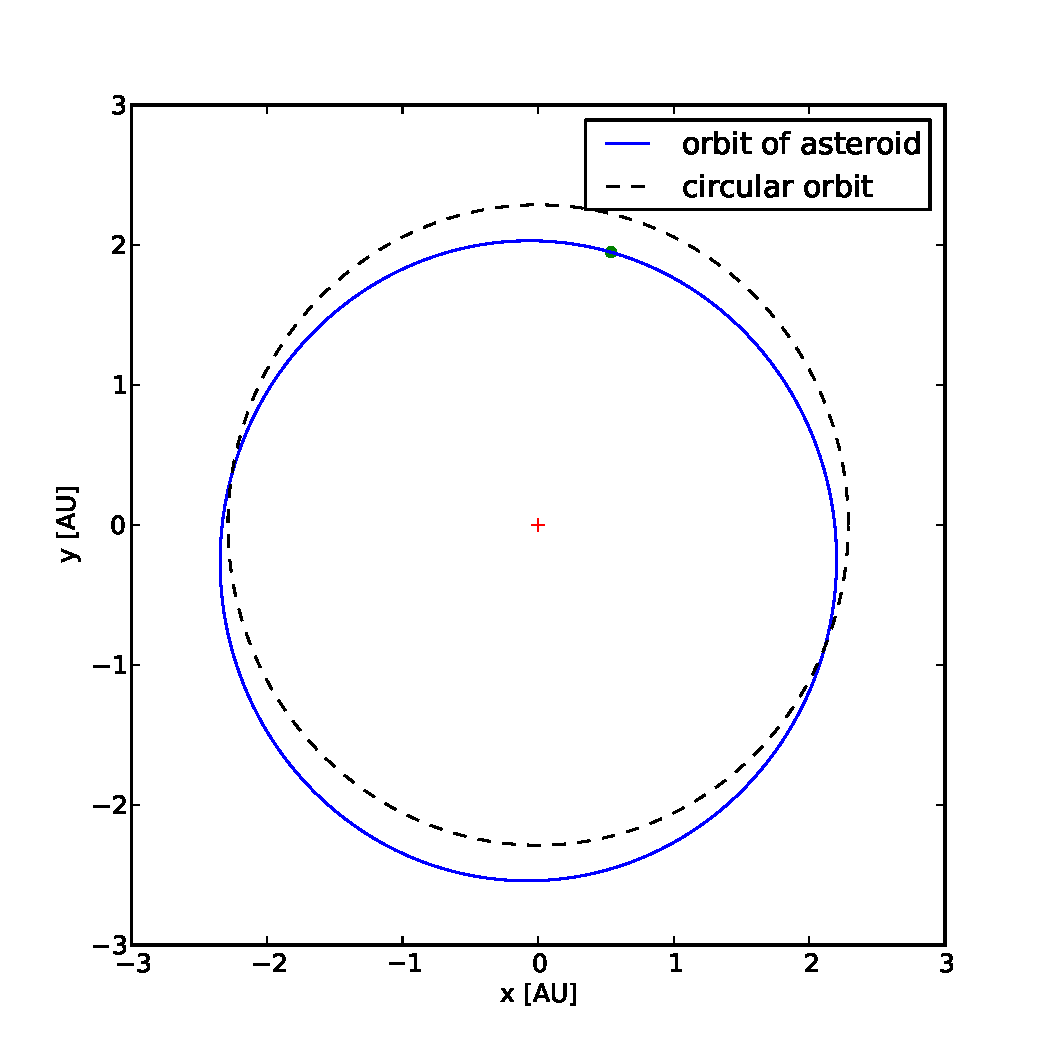
\includegraphics [angle=0,height=7cm,width=7cm]{pic/urania_orbit.pdf} 
\caption{Full orbit of Urania compared with a circular orbit, which has Sun in the center. The green dot on the orbit of Urania is the point where perihelion occurs.}
\label{fig:orbit}
\end{figure}
%~~~~~~~~~~~~~~~~~~~~~~~~~~~~~~~~~~~~~~~~~~~~
In figure \ref{fig:orbit}, it is clear that the perihelion occurs where the orbit is closer to the center, that is, the Sun. 


\subsection{Predicting positions}
\label{sec:predict}
Using the equation from equation \ref{eq:orbital0}, \ref{eq:orbital1} and \ref{eq:orbital2}, the position was predicted for the same five epoch so that it was easy to compare and check for the accuracy, see Appendix B for code. Following is the table that shows the predicted results. 
%~~~~~~~~~~~~~~~~~~~~~~~~~~~~~~~~~~~~~~~~~~~~
\begin{table}[H]
\centering % used for centering table
\caption{Comparing predicted Right Ascension and Declination of Urania over 5 epochs with JPL.}
\tabcolsep 2.pt %\small
\footnotesize
\begin{tabular}{ccccccc}% centred columns (8 columns)
\hline
\hline
Date  & $\alpha$ & $\delta$ & $\Delta \alpha$ & $\Delta \delta$ \\
& [hms J2000]&[dms J2000] &[hms J2000]&[dms J2000]\\
\hline
\hline
20 &2:53:38.01& +19:55:29.73&0:04:11.18 &0:19:00.87\\
21 &2:55:17.43& +19:02:28.03&0:03:27.03 &0:14:18.07\\
23 &2:58:37.80& +19:16:18.51&0:02:03.50 &0:05:21.09\\
24 &3:00:18.63& +19:23:10.57&0:01:18.82 &0:00:53.11\\
29 &3:07:06.53& +19:50:16.47&0:00:04.89  &0:11:57.07\\


\hline
\hline
\end{tabular}
\label{table:prediction} % is used to refer this table in the text
\end{table}
%~~~~~~~~~~~~~~~~~~~~~~~~~~~~~~~~~~~~~~~~~~~~
From Table \ref{table:prediction}, the results show that error in $\alpha$ is decreasing where as error in $\delta$ are much random. After plotting the JPL position and predicted positions over time, the results are as following:

\begin{figure}[H]
\centering
	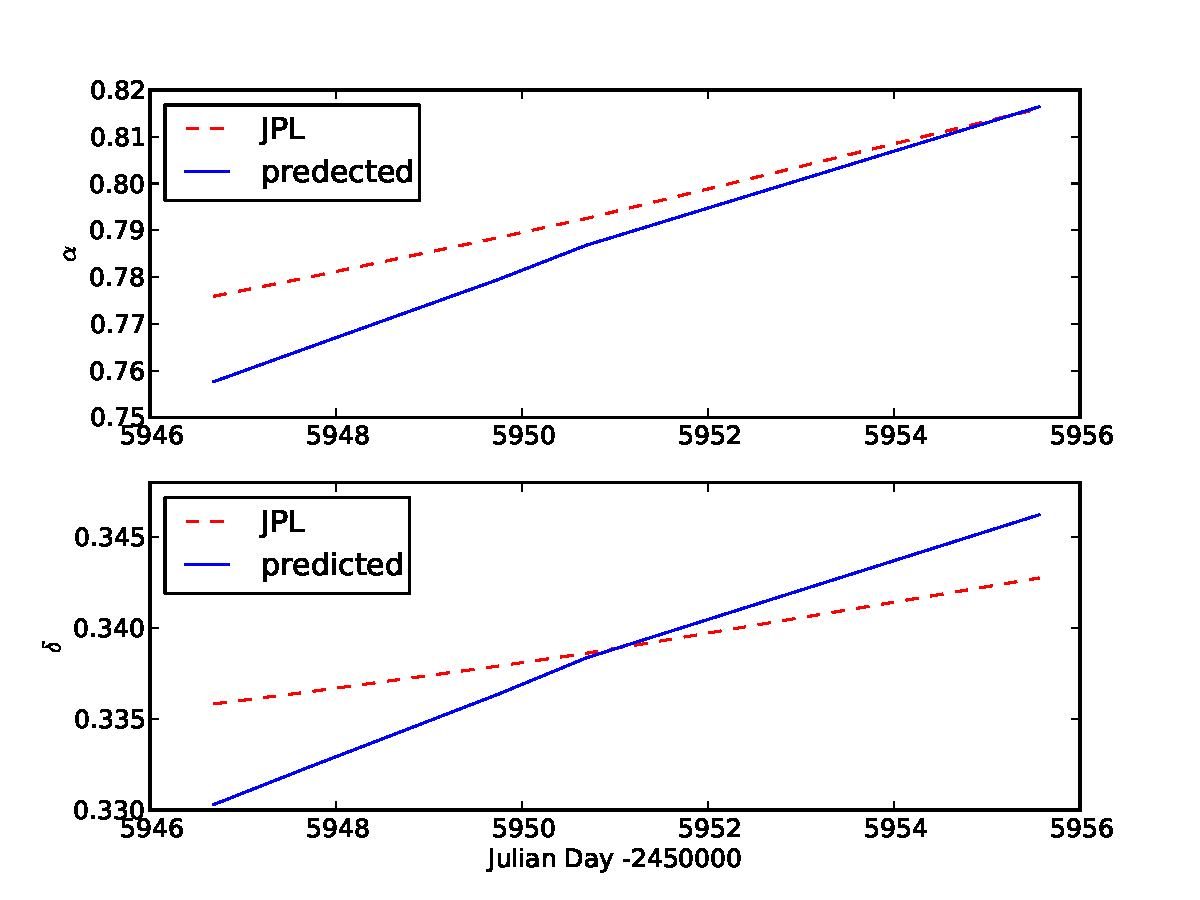
\includegraphics [angle=0,height=7cm,width=10cm]{pic/predicted.pdf} 
\caption{Predicted position and JPL position vs. time}
\label{fig:orbit}
\end{figure}
Here, it is clear that there is lot of variation in error. However, the answer is still quite close to the actual results. Here the angles  was converted using the loops in python, see Appendix C for code.
%###########################################################################################################################################################################

%####################### Discussion 
\section{Discussion}
\label{sec:discuss}
\subsection{Saturated Data}
\label{sec:saturated}
When calculating $r$ and $\rho$ there was a problem. The convergence of $\rho$ was 0, which as mentioned in Section \ref{sec:r_rho} mean that distance between Urania and Earth is 0. Clearly, that is not the case. Therefore, as a solution, JPL position during those epoch were used. However, its quite bizarre that while one works, the other does not, especially with such small errors. The explanation is that errors were not small. In calculating orbital elements, at least three position of the astroid at three different epoch are required with very high accuracy. In table \ref{table:position}, errors on right ascension are quite small with a exception of $29^{th}$ one. However, the errors on the declination are quite huge for two of them: $21^{st}$ and $23^{rd}$. This errors is then propagated through out rest of the calculations and give the result of $\rho$ = 0 and $r$ = 1. This errors was tried to be reduced but because the $\chi_{red}^2$ value is quite high, as mention is Section \ref{sec:position}. It's quite hard to reduce the errors even more. Once conclusion that can be made from this is that the data is saturated. And deriving plate constants on it would be quite hard. 
\subsection{Predictions}
\label{sec:errorpridiction}
Another thing that was curious was prediction. Even after using JPL for deriving orbital elements, the predictions for the same epoch were quite off, as it can be seen in Table \ref{table:prediction} and Figure \ref{fig:prediction}. For right ascension the values are converging to the correct value as the time goes by. However, the declination is crossing it, as if it has different motion. This could be the result of errors propagating though various calculations. Also, there were some assumptions and approximations that was made. Assumption being neglecting the effect of Jupiter and asteroids in the similar orbit. We only took three bodies under consideration: Sun, Earth and Urania. And the approximation was the use of taylor exception, which create errors that are then propagate through rest of the calculations. 

\begin{appendices}
\section{Calculating $\rho$ and $r$ }

\begin{lstlisting}
# function for calculating rho
def rho_calc (k, RR, r,R,s,sd,sdd):
    rho = (k**2)*((1/RR**3)-(1/r**3))*(np.dot(sd,(np.cross(R,s))))
            /(np.dot(sd,(np.cross(sdd,s))))
    return rho

# function for calculating r
def r_calc (rho, RR, R, s ):
    r = np.sqrt((rho**2)+(RR**2) + (2*rho*(np.dot(R,s))))
    return r

# this is used to get the values for rho and r
rho = 0.1 # initial value
r = 0.1 # initial value

m = 0
rlist = np.zeros(101) 
rlist[0] = r
rholist = np.zeros(101)
rholist[0] = rho
while m < 100:
    r = r_calc (rho, RR, R, s )
    rlist[m+1] = r
    rho = rho_calc (k, RR, r,R,s,sd,sdd)
    rholist[m+1] = rho
    m+=1
\end{lstlisting}
This piece of code was used to calculate the $r$ and $\rho$ value by iterating over 100 increments to get a convergence. This failed for the position values obtained from the data set but worked for JPL positions. 

\section{Predicting the position at given time}
\begin{lstlisting}
timehold = [2455946.68646, 2455947.69476, 2455949.73866, 
            2455950.68528, 2455955.56062]
r_vec = []
r_eq = []
RA = [] # this will store right accession values
DEC = [] # this will store declination values
for time in timehold:
    holdindex = np.nonzero(t<=time) # store all the index 
                            #from array t,until the element 
                            #value is less than or equal to time
    MAnomaly = n*(time - tau)
    EAnomaly = E[holdindex[0][-1]] 
    trueAnomaly = find_v(e,EAnomaly)
    theta_predict = trueAnomaly+w
    r_predict = a*(1-e*np.cos(EAnomaly))
    rvec = np.matrix([(r_predict*np.cos(theta_predict)),
                    (r_predict*np.sin(theta_predict)),
                    0])
    recliptic = (TzTx*rvec.T)
    Te = np.matrix([[1,0,0],
                    [0, np.cos(epislon), -np.sin(epislon)],
                    [0, np.sin(epislon), np.cos(epislon)]])
    requatorial = np.array((Te*recliptic).T)
    recliptic = np.array(recliptic.T)
    
    Rvec = np.array((Te*np.matrix(R).T).T)
    rho_s = recliptic - R
    rho_s2 = Te*np.matrix(rho_s).T
    rho_s = np.array(rho_s2.T)
    rho = np.linalg.norm(rho_s)
    
    r_a = np.arctan(rho_s[0][1]/rho_s[0][0])
    dec = np.arcsin(rho_s[0][2]/rho)
    RA.append(r_a)
    DEC.append(dec)
    r_vec.append(rvec)

\end{lstlisting}
The method is straight forward. Except obtaining the value for EAnomaly. This was done by finding the index of where that time occurs in array t (see the code for holdindex). And then find the corresponding Eccentric Anomaly using the last value of holdindex.

\section{Converting time to radian and visevera}
This loop was used to convert standard position to radians
\begin{lstlisting}
ra = []
dec = []
for i in list:
    r = 15*(float(i[0]) + float(i[1])/60. 
        + float(i[2])/3600.)*np.pi/180
    d = (float(i[3]) + float(i[4])/60. 
        + float(i[5])/3600.)*np.pi/180
    ra.append(r)
    dec.append(d)
\end{lstlisting}

This loop was used to convert radians to standard position
\begin{lstlisting}
ra_new = []
dec_new = []
j = 0
while j < len(RA):
    a1 = RA[j]*180/(np.pi*15)
    a2 = a1%1
    a3 = a2*60%1
    a4 = a3*60
    alpha = [a1-a2,a2*60-a3,a4]
    
    d1 = DEC[j]*180/np.pi
    d2 = d1%1
    d3 = d2*60%1
    d4 = d3*60
    delta = [d1-d2,d2*60-d3,d4]
    
    ra_new.append(alpha)
    dec_new.append(delta)
    j+=1
\end{lstlisting}

\end{appendices}

\bibliographystyle{plain}
\bibliography{references.bib}
\end{document}
